
%----------------------------------------------------------------------------------------
% SECTION 1
%----------------------------------------------------------------------------------------

\section{Training Data}
\label{train_data}


%-----------------------------------
% SUBSECTION 1
%-----------------------------------
\subsection{Data simulation}

The spectra were simulated with the Software Sessa v2.2.0 developed by Smekal and others. It uses binding energies from the NIST database and inelastic mean free paths (IMFPs) from various publications and simulations to calculate the spectra. Since version 2.2.0, it also accounts for energy dependence of the IMFP \cite{noauthor_nist_2010}.
Sessa includes Photoelectron peaks and Auger-Electron peaks, but does not always include multiplet splitting. Furthermore, it lacks the specific shape-parameters of many Auger-Electron peaks to simulate them correctly.

As the probing depth of XPS is around 5-10 nanometers and the information diminishes rapidly after the first few nanometers, the thicknesses used for simulation of the top layer are n $\in$ [1, 2, 3, 4, 5] nm. A second simulation approach was to simulate slow transitions of elements such as seen in migration, oxidation or alloying processes. As shown in \ref{fig:layers} b), two components are used in a mixture across the lateral cross-section. While one component decreases from 100\%, the other one increases symmetrically.

\begin{figure}
    \centering
    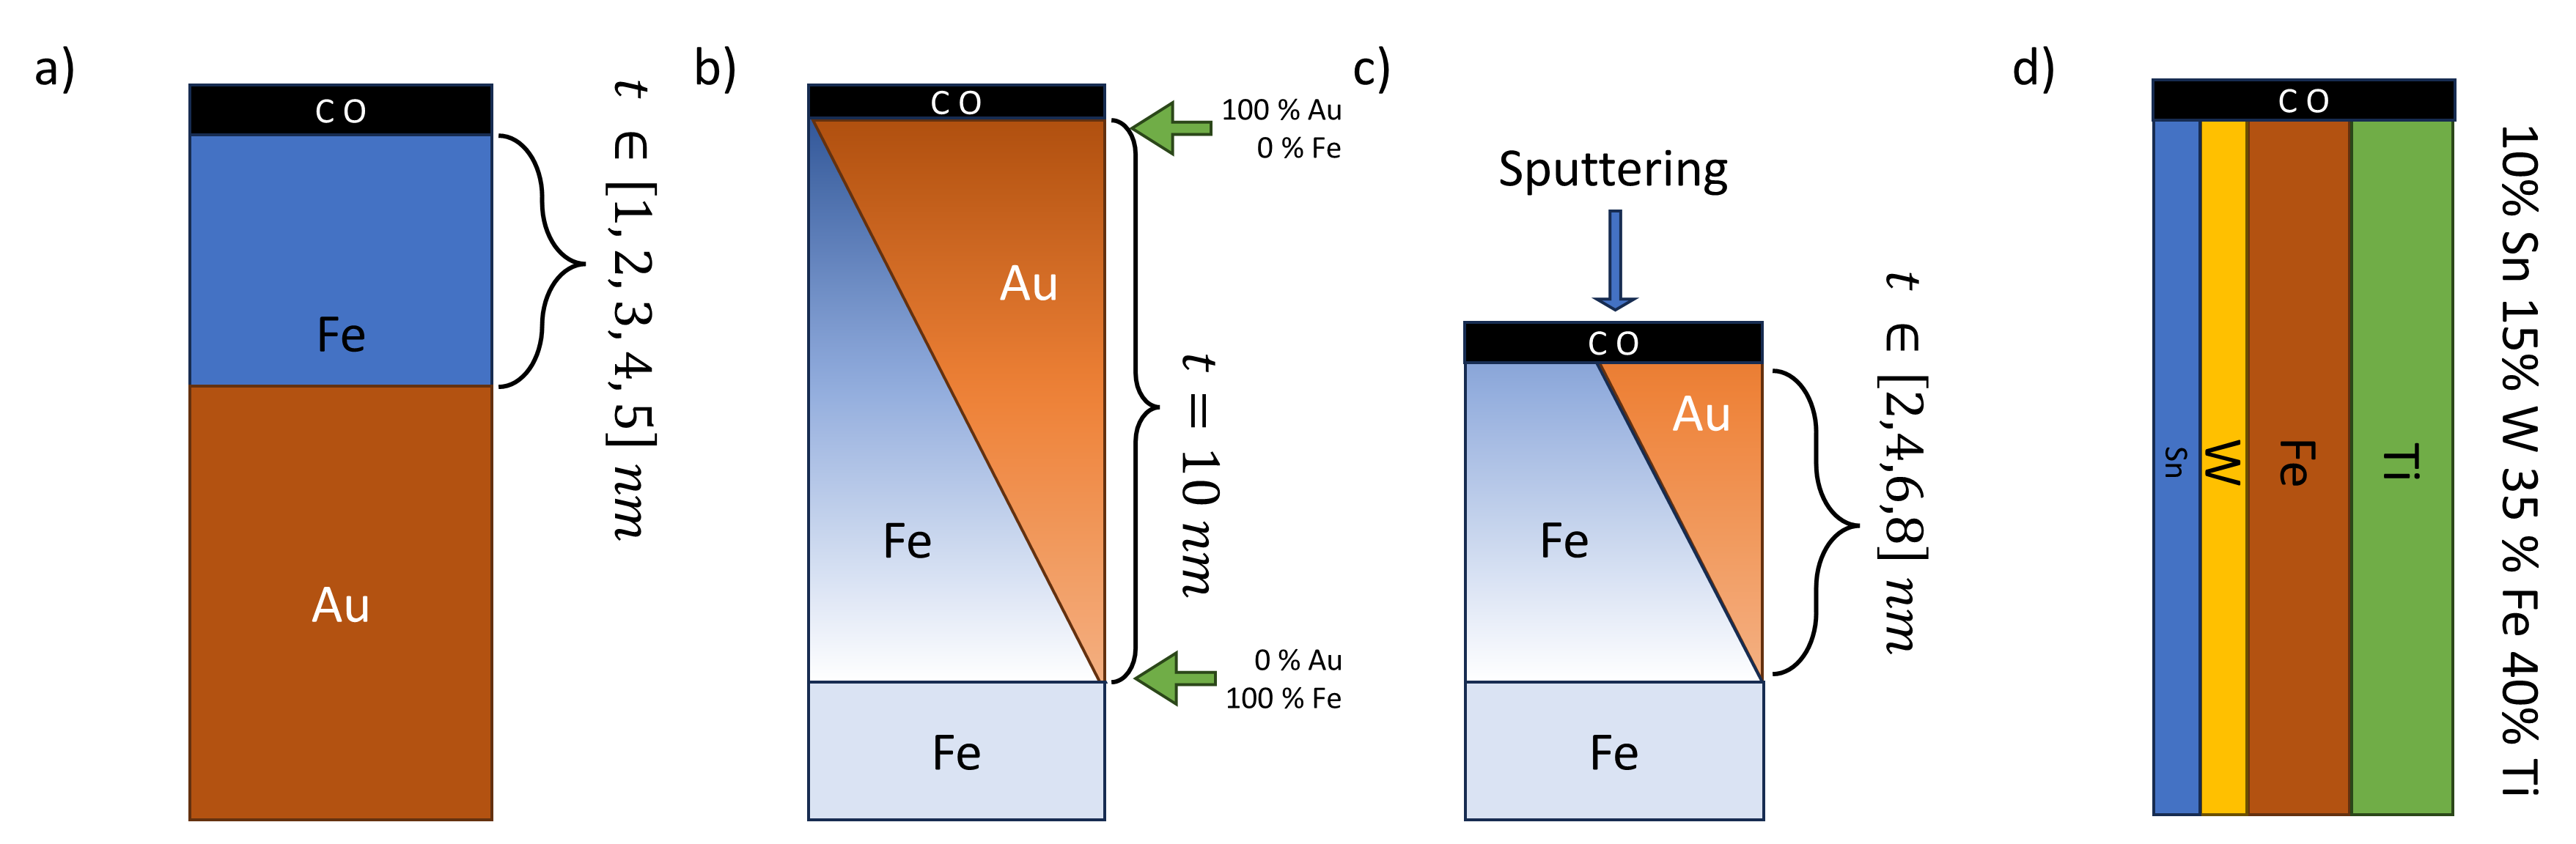
\includegraphics[width=\textwidth]{Figures/layers.png}
    \caption{Schematic figure of different layered systems simulated a) separated layers with defined top layer thickness, b) top layer with a concentration gradient and thickness 10 nm, c) sputtered version of b) where the top layer thickness is reduced, d) multi-component one-layer system}
    \label{fig:layers}
\end{figure}


The spectra simulated are using two components from all elements (n=81), thus 6'480 permutations without repetition. With the five thicknesses, we obtain 32'400 spectra for each experimental setup a) and b)+c). Additionally, single-component systems were simulated consisting of one bulk element (top and bottom layer equal). The contamination layer is often seen on uncleaned samples but, as discussed, does not resemble a factual layer in XPS analysis. As the contamination has diverse provenance, datasets were constructed with and without a contamination layer. They are denoted as cont and clean, respectively. Finally, both datasets were used to provide the model with variations of contaminated and clean samples, which is denoted as \emph{mixcont} (n=97k).

In the \emph{cont} dataset, to achieve a similar carbon and oxide content as experimental data, there are two versions with a carbon and oxide layer (CO) once with a thickness between 12 and 24 with mode 15 Angstrom and once with 6 Angstrom thickness on top. This was chosen to imitate a slight and a severe contamination. An example comparison of experimental and simulated and preprocessed data is shown in Figure \ref{fig:ex_vs_sim}. Firstly, it is obvious that the background was not accurately modelled as shown in detail (a), as the experimental background increases gradually, whereas one of the modelled background decrease and the other is negligible throughout. Further, the Auger-Peak shape (denoted as Fe Auger-Peak) from the simulated data does not correspond to the observed one. Most importantly, we see the inconsistency of the modelling of the contamination. It is obvious that we have too much inelastic background intensity with the contamination layer and too few without, thus we would expect better performance on experimental data when a model is trained with the mixcont dataset.

\begin{figure}[H]
    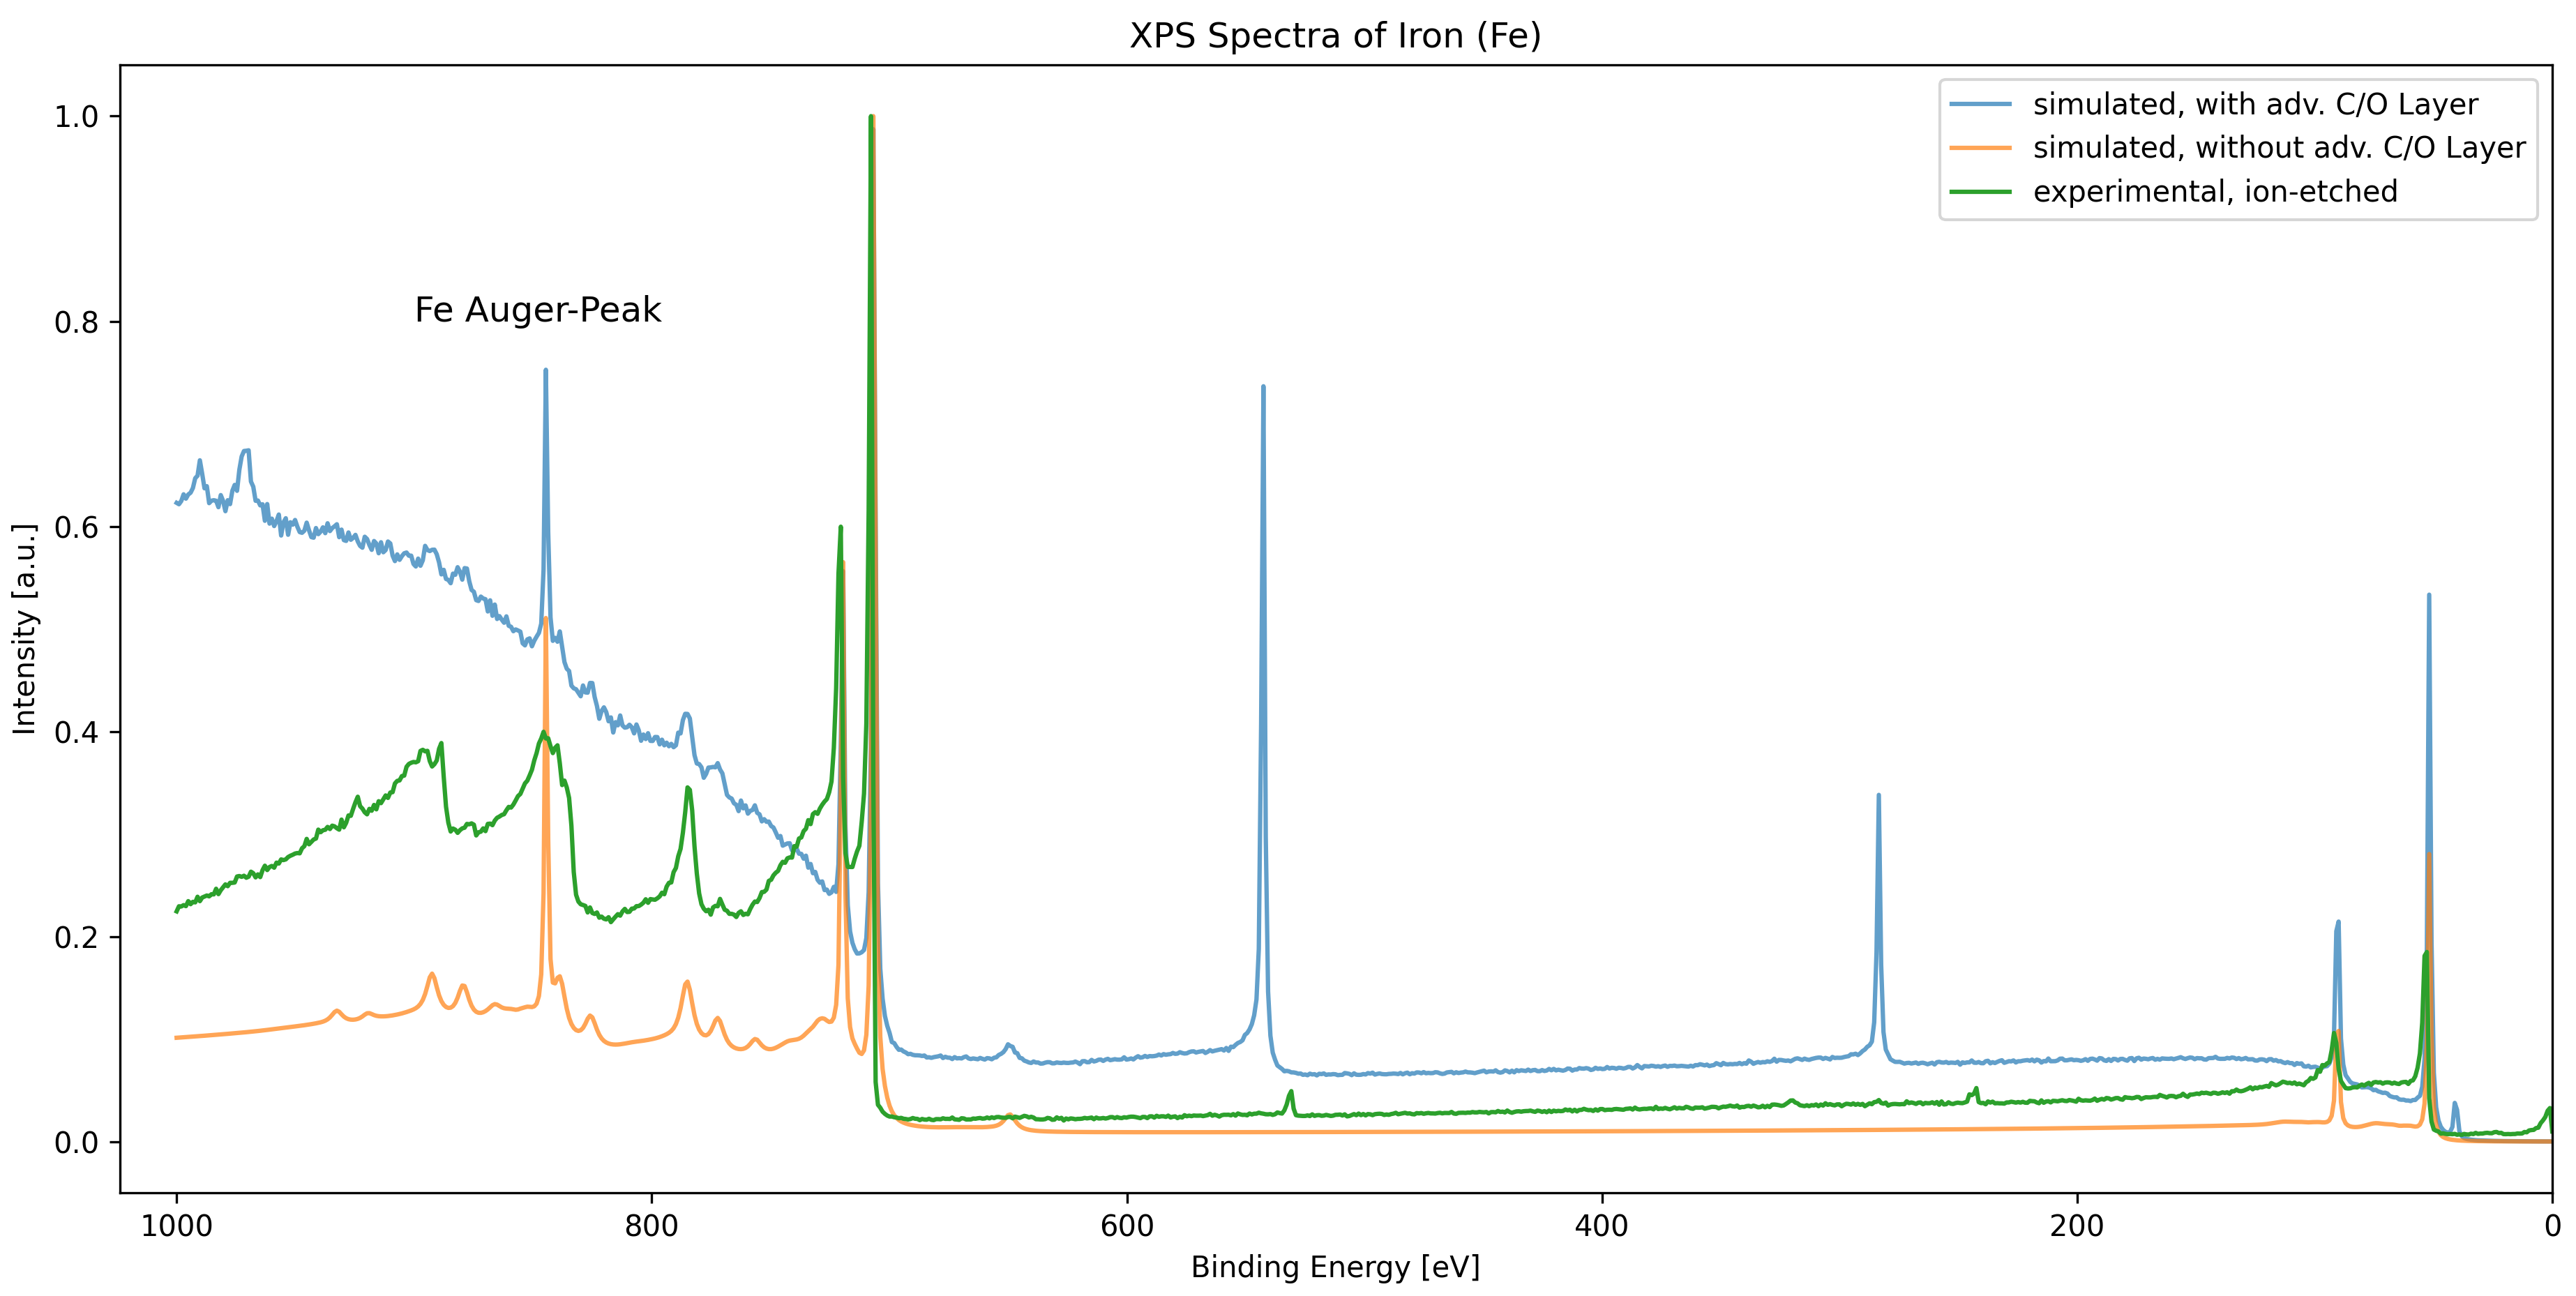
\includegraphics[width=\textwidth]{Figures/Fe_XPS.png}
    \caption{Comparison of experimental \& preprocessed vs simulated spectra of elemental iron}
    \label{fig:ex_vs_sim}
    \centering
\end{figure}

For the experimental setup d), we assumed that the Spectra of mixed compounds is comparable to the Spectra of the elemental constituents in the corresponding ratios. It must be noted that this is not true, because as elements form a compound, they undergo connections with their valence electrons which - at least - changes the valence-band photoelectron peak positions. However, this simplification allows us to easily simulate thousands of spectra somehow similar to the spectra we would measure. For this mixed-component model, 30k spectra were generated with a content of 5 - 60 \% for each component, with two to four components in total. As - when components undergo bonds - we observe chemical shifts in the spectra for the specific orbital peaks of the components, these were included in the model as explained later in this chapter.
 
To simulate, the command-line-interface feature of Sessa was used, which is documented in their users guide \cite{werner_simulation_2021}. It allows users to interact with the software through a file of commands which are then sequentially read and processed. The commands were first built, saved to a text-file and then read and processed with Sessa using the python subprocess module. To allow diverse simulation properties, classes for Experiments and Layers were defined. Furthermore, functions for the simulation, finding and setting chemical shifts, as well as writing the session file were programmed. The corresponding code can be found in Appendix \ref{Sessa_Module}.

Because the Sessa software didn't allow reading the chemical shift database from the command line interface, the NIST database was webscraped and saved as a readable database - the code can be found in Appendix \ref{NIST_WebScraper}. Unfortunately, the database has entries with wrong energy descriptions (kinetic/binding energy) and thus, anything deviating more than 10\% from the median or the original peak position was converted to the opposite measure.
For each mixture compound simulated according to model d), a fuzzy string matching was performed and the best match was taken with a certain probability $p$.


%-----------------------------------
% SUBSECTION 2
%-----------------------------------

\subsection{Data preprocessing}

Each spectra was max-normalized using equation \ref{eqn:normalize}, where each component $x$ is divided by the maximum component of the spectra. Using the max-normalization ensures that any background-shift of the whole spectrum is kept as a feature.
\begin{equation}
    x' = \frac{x}{max(x)}
\label{eqn:normalize}
\end{equation}
Additionally to the normalization, a random percentage of 0.1, 0.2 or 0.3 \% relative noise was added to mimick the noise usually observed in XPS spectral data. The code for the preprocessing of all datasets is provided in Appendix \ref{train_data_generation}.